%%=======================================================================
% !Mode:: "TeX:UTF-8"
% !TEX program  = xelatex
%%=======================================================================
% 模板名称：thubeamer
% 模板版本：V1.1.0
% 模板作者：杨敬轩（Jingxuan Yang）
% 联系作者：yangjx20@mails.tsinghua.edu.cn & yanglatex2e@gmail.com
% 模板适用：清华大学风格 Beamer 模板
% 模板编译：手动编译方法参看 README.md 或 thubeamer.pdf
%          编译 beamer 之前必须编译说明文档：make doc 或双击 makedoc.bat
%          编译说明文档同时分离出四个样式文件 *thubeamer.sty
%          更新信息：2021/11/15
%%=======================================================================
% ============================================================
% 《Web前端技术实训》2026 夏 —— 课程大作业答辩
% SmartCinema 智能影院选座系统
%
% 章节结构（对应答辩要求）：
%   1. 小组分工                 （内容进行中）
%   2. 核心技术设计
%   3. 系统演示                 （仅结构，内容 TODO）
%   4. 项目总结与心得           （内容进行中）
%
% ============================================================

% 使用本机可用的中文字体；在 XeLaTeX 下显式配置，避免模板默认 Windows 字体集。
\PassOptionsToPackage{fontset=none}{ctex}

% 设置文档类别为 <beamer>
% \documentclass[aspectratio=169]{beamer} % 设置长宽比为 16:9
\documentclass{beamer}

% 使用 <thubeamer> 主题
% 模板选项如下
% (a.1) smoothbars: 页面顶端单行显示目录，默认选项
\usetheme{thubeamer}

\setCJKmainfont{Songti SC}
\setCJKsansfont{Heiti SC}
\setCJKmonofont{Songti SC}

% (a.2) sidebar: 页面左侧分栏显示目录
% \usetheme[sidebar]{thubeamer}

% (b) sectiontoc: 在每节（section）前显示目录，并高亮显示当前节，默认不显示

% (c) subsectiontoc: 在每小节（subsection）前显示目录，并高亮显示当前节和当前小节，默认不显示

% (d) en: 仅使用英文来制作 beamer，应用此选项后，汉字将全部无法编译

% 图片存放路径
\graphicspath{{figures/}}
\usetikzlibrary{positioning,calc}

\include{macros}

% 封面信息，方括号内容是显示在左侧边栏的内容（当选择 sidebar 主题时有效）
% TODO: 将 XXX 替换为真实姓名 / 学号
\title[SmartCinema]{SmartCinema 智能影院选座系统\\[2mm] 课程大作业答辩}
\author[豆浆糖油饼]{答辩人：王博翰，潘宇治，赵常景行，杨世威}
\institute[清华大学]{\small 清华大学未央书院}
\date{\small \vskip -10pt 2026 年 8 月}

% 开始写文章
\begin{document}

% 标题页
\begin{frame}
	\maketitle
\end{frame}

% 目录页
\section*{目录}
\frame{
  \frametitle{\secname}
  \tableofcontents[hideallsubsections]
}

%%=======================================================================
%% 1. 小组分工
%%=======================================================================
\section{小组分工}

\subsection{成员信息}

\begin{frame}{成员信息}
  \begin{table}[htbp]
    \small
    \centering
    \begin{tabular}{cp{0.2\textwidth}p{0.28\textwidth}p{0.25\textwidth}}
      \toprule
      序号 & 姓名 & 学号 & 角色 \\
      \midrule
      1 & 王博翰 & 2024012510 & 组长 \\
      2 & 潘宇治 & 2024012509 & 组员 \\
      3 & 赵常景行 & 2024012513 & 组员 \\
      4 & 杨世威 & 2024012512 & 组员 \\
      \bottomrule
    \end{tabular}
  \end{table}
\end{frame}

\subsection{分工与职责}

\begin{frame}{分工与职责}
  \begin{columns}[T,onlytextwidth]
    \column{0.54\textwidth}
      \begin{table}
        \footnotesize
        \centering
        \begin{tabular}{p{0.22\textwidth}p{0.63\textwidth}}
          \toprule
          成员 & 负责模块 \\
          \midrule
          王博翰 & 初始框架与开发流程设计、PPT 制作 \\
          杨世威 & 第二版测试与优化 \\
          潘宇治 & 第三版后续开发、PPT 制作 \\
          赵常景行 & 第四版后续开发、PPT 制作 \\
          \bottomrule
        \end{tabular}
      \end{table}
    \column{0.42\textwidth}
      \begin{block}{协作方式}
        \small
        \begin{itemize}
          \setlength{\itemsep}{7pt}
          \item Git + GitHub 远程协作
          \item 功能分支 $\rightarrow$ PR 评审\\测试集成后合入 \texttt{main}
        \end{itemize}
      \end{block}
  \end{columns}
\end{frame}

%%=======================================================================
%% 2. 系统演示
%%=======================================================================
\section{系统演示}

\subsection{现场演示}

\begin{frame}{现场演示}
  \begin{block}{演示流程}
    \begin{enumerate}
      \setlength{\itemsep}{4pt}
      \item 注册 / 登录 $\rightarrow$ 进入主界面
      \item 选择放映厅 $\rightarrow$ 智能推荐选座 / 手动选座
      \item 查看体验评分与热度地图 $\rightarrow$ 下单
    \end{enumerate}
  \end{block}
\end{frame}

%%=======================================================================
%% 3. 实现亮点
%%=======================================================================
\section{实现亮点}

\subsection{前端 UI 分层}

\begin{frame}{双 Canvas 与语义 DOM 分层}
  \begin{columns}[T,onlytextwidth]
    \column{0.43\textwidth}
      \begin{block}{设计需求}
        \small
        \begin{itemize}
          \setlength{\itemsep}{6pt}
          \item 热度和座位状态的更新频率不同
          \item 100--300 个座位需要保持绘制流畅
          \item Canvas 本身不支持 DOM 语义
        \end{itemize}
      \end{block}
    \column{0.54\textwidth}
      \centering
      \begin{tikzpicture}[font=\small, node distance=5mm]
        \node[draw=purple!80!black, fill=purple!10, rounded corners, align=center,
          minimum width=48mm, minimum height=12mm] (semantic)
          {\textbf{语义 DOM 层}\\ARIA 信息、键盘导航、读屏操作};
        \node[draw=purple!80!black, fill=purple!10, rounded corners, align=center,
          below=of semantic, minimum width=48mm, minimum height=12mm] (seat)
          {\textbf{座位 Canvas}\\座位绘制、选中状态、点击与框选};
        \node[draw=purple!80!black, fill=purple!20, rounded corners, align=center,
          below=of seat, minimum width=48mm, minimum height=12mm] (heat)
          {\textbf{热度 Canvas}\\高斯插值、低分辨率位图、缓存};
        \draw[->, thick, purple!80!black] (semantic) --
          node[right, font=\scriptsize] {共享座位状态} (seat);
        \draw[->, thick, purple!80!black] (seat) -- (heat);
      \end{tikzpicture}
  \end{columns}
  \vspace{5mm}
  \begin{minipage}{\textwidth}
    \centering\footnotesize
    三层共享座位状态，分别负责热度计算、交互绘制与无障碍操作。
  \end{minipage}
\end{frame}

\begin{frame}{液态玻璃容器的 CSS 分层实现}
  \centering
  {\small 网页整体设计参考苹果的“液态玻璃”风格}\\
  {\small 在 Web 端将一个容器拆成四个 CSS 层。}

  \vspace{3mm}
  \begin{tikzpicture}[font=\scriptsize, node distance=2.4mm]
    \node[draw=purple!80!black, fill=purple!10, rounded corners, align=center,
      minimum width=23mm, minimum height=11mm] (background)
      {\textbf{背景环境}\\渐变与光斑};
    \node[draw=purple!80!black, fill=purple!10, rounded corners, align=center,
      right=of background, minimum width=23mm, minimum height=11mm] (material)
      {\textbf{半透明材质}\\背景与滤镜};
    \node[draw=purple!80!black, fill=purple!10, rounded corners, align=center,
      right=of material, minimum width=23mm, minimum height=11mm] (edge)
      {\textbf{边缘与深度}\\高光与阴影};
    \node[draw=purple!80!black, fill=purple!20, rounded corners, align=center,
      right=of edge, minimum width=23mm, minimum height=11mm] (content)
      {\textbf{容器内容}\\文字、工具栏、Canvas};
    \draw[->, thick, purple!80!black] (background) -- (material);
    \draw[->, thick, purple!80!black] (material) -- (edge);
    \draw[->, thick, purple!80!black] (edge) -- (content);
  \end{tikzpicture}

  \vspace{3mm}
  \begin{columns}[T,onlytextwidth]
    \column{0.38\textwidth}
      \begin{block}{CSS 示例}
        \ttfamily\fontsize{6.5}{7.5}\selectfont
        .glass \{\\
        \quad background:\\
        \qquad rgba(255,255,255,.1);\\
        \quad backdrop-filter:\\
        \qquad blur(22px)\\
        \qquad saturate(112\%) contrast(104\%);\\
        \}
      \end{block}
    \column{0.59\textwidth}
      \begin{block}{实现对应}
        \scriptsize
        \begin{itemize}
          \setlength{\itemsep}{2pt}
          \item \texttt{background}：半透明渐变填充
          \item \texttt{backdrop-filter}：模糊、饱和度与对比度
          \item 伪元素 + \texttt{mask}：表面高光与渐变边缘
          \item \texttt{box-shadow}：外部阴影与内部高光
          \item 媒体查询：实色回退与高对比显示
        \end{itemize}
      \end{block}
  \end{columns}

  \vspace{4mm}
  \begin{minipage}{\textwidth}
    \centering\footnotesize
    滤镜与核心交互解耦：不可用或降低透明度时，仅将材质回退为实色容器。
  \end{minipage}
\end{frame}

\begin{frame}{界面实现效果}
  \centering
  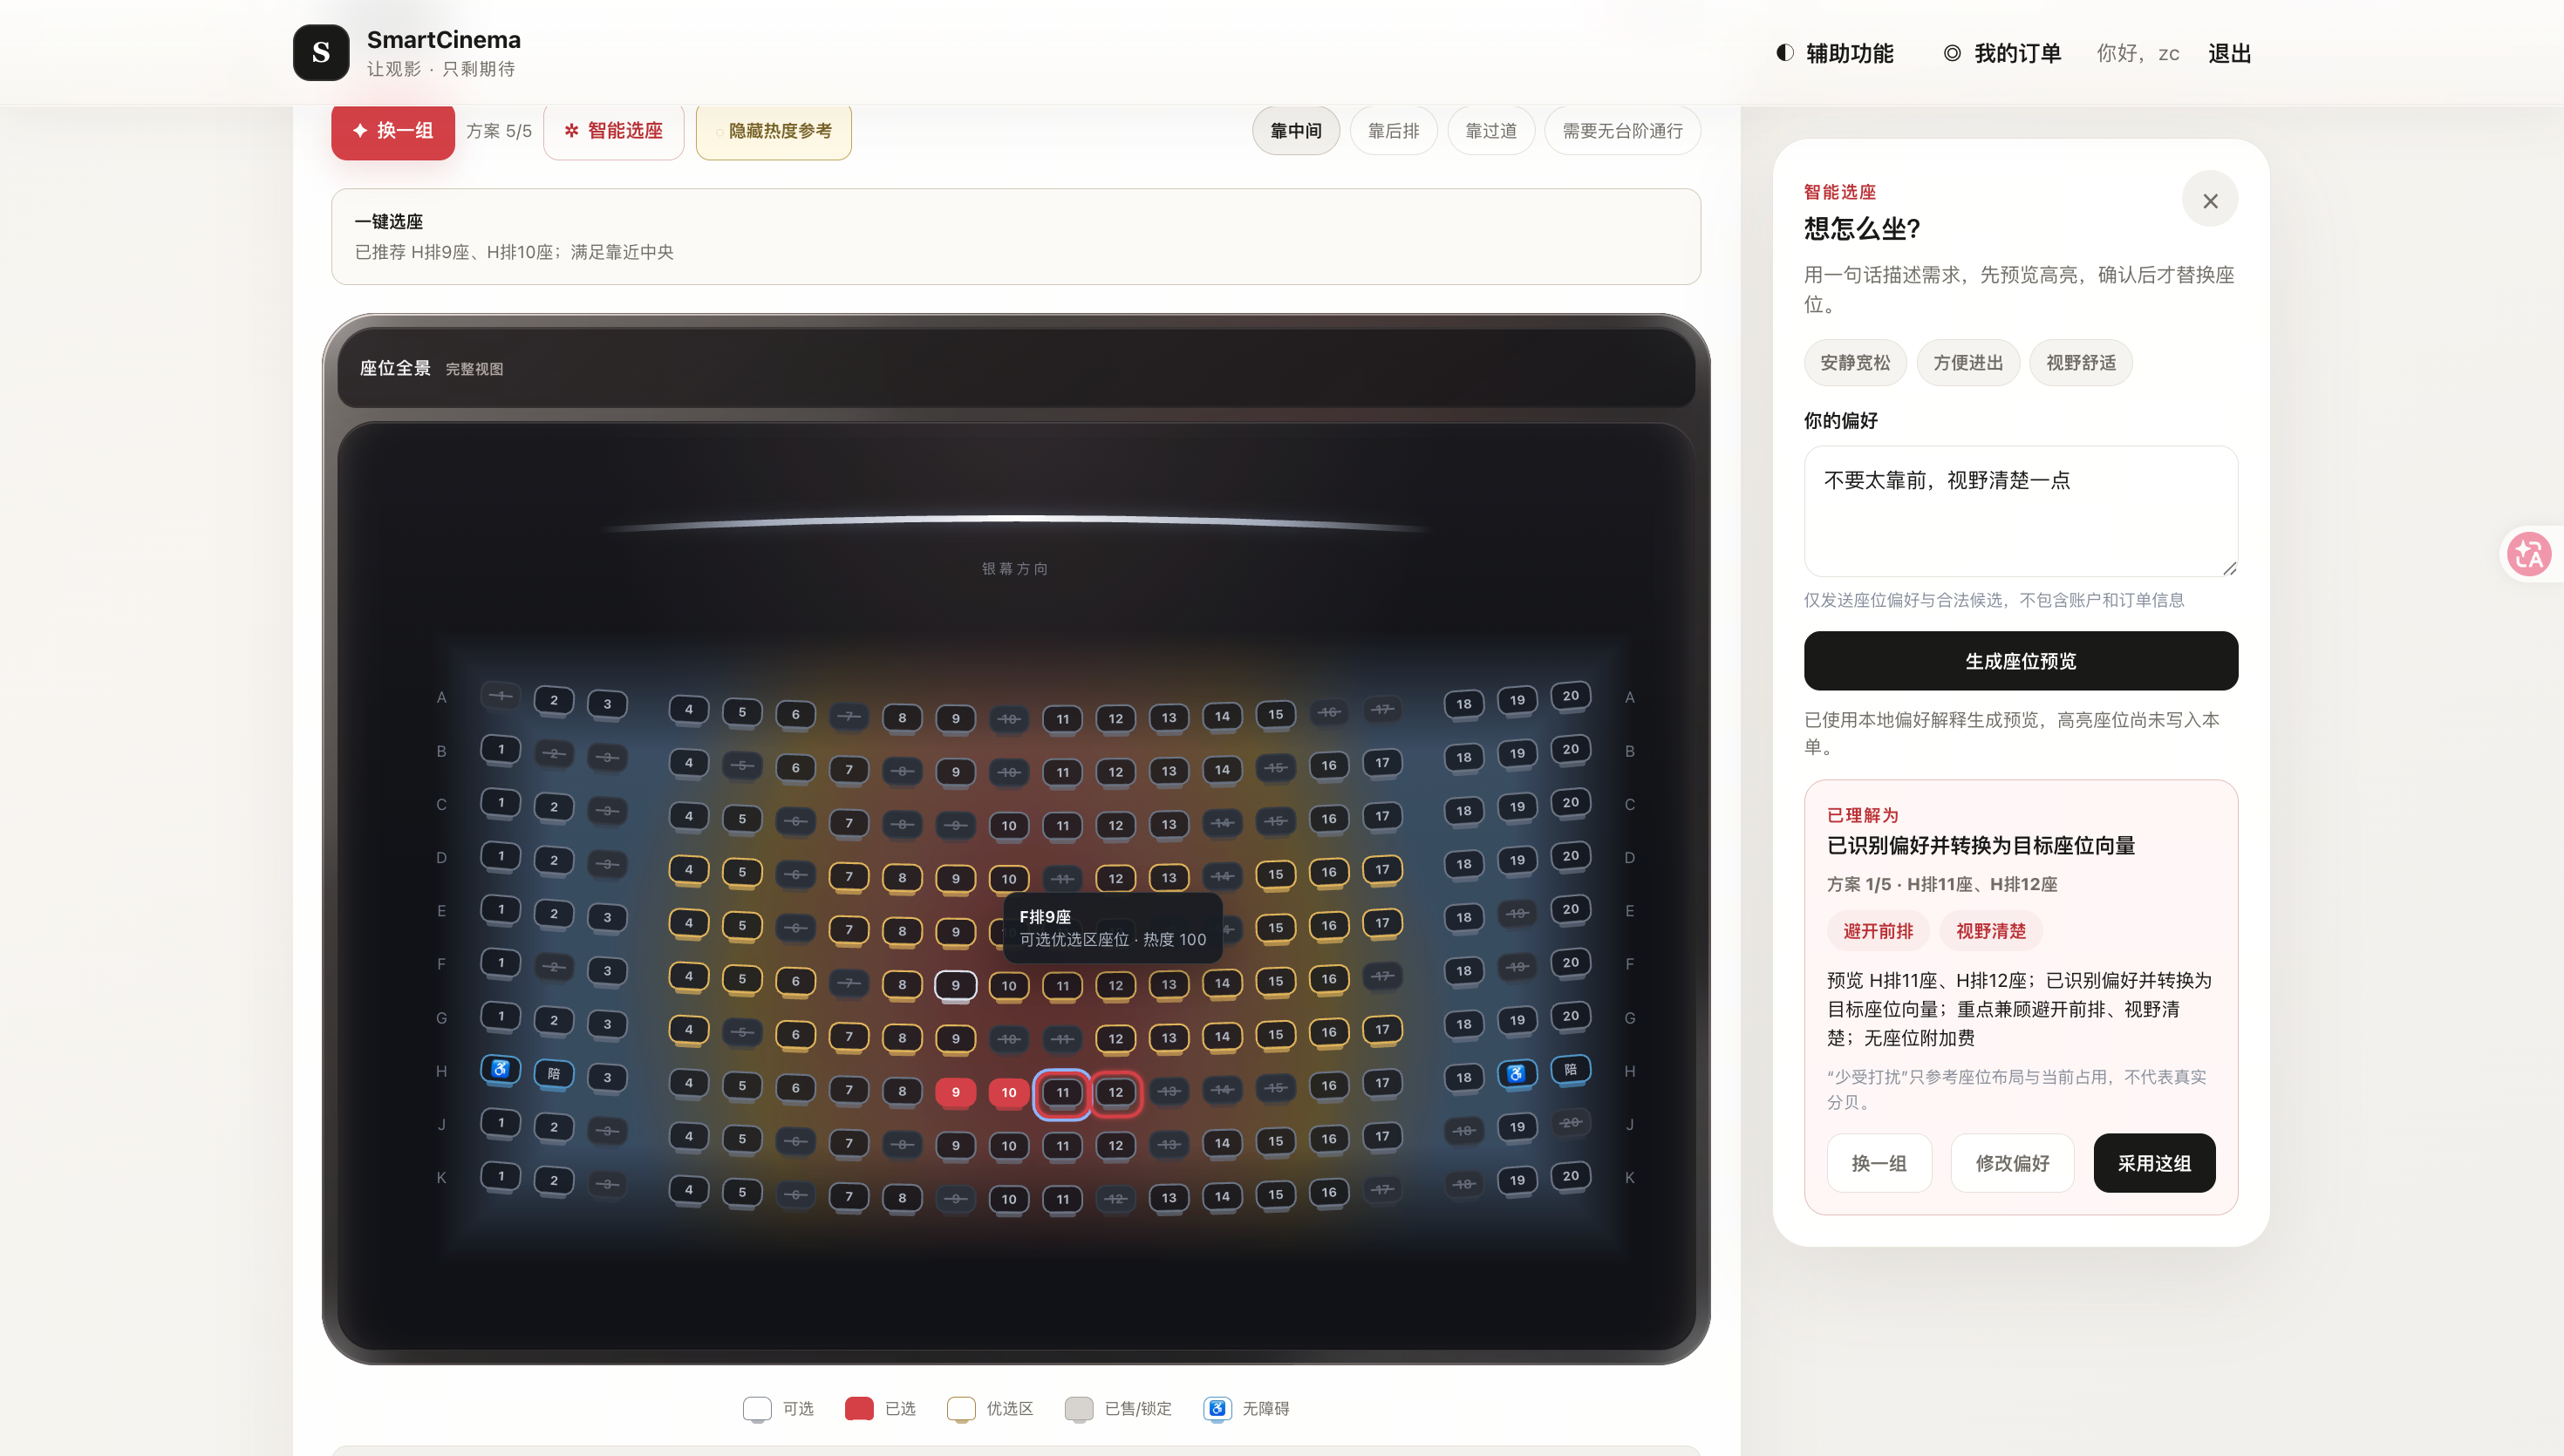
\includegraphics[trim=300 80 300 0,clip,
    width=\textwidth,height=0.85\textheight,keepaspectratio]{UI.png}
\end{frame}

%%=======================================================================
%% 4. 项目总结与心得
%%=======================================================================
\section{项目总结与心得}

\subsection{项目过程中遇到的问题及解决方案}

\begin{frame}{遇到的问题及解决方案}
  \begin{block}{问题}
    \begin{itemize}
      \setlength{\itemsep}{4pt}
      \item \textbf{AI 选座语义失真}：六维“好坏分”无法区分“太近”和“太远”；近视用户想靠前时，反而可能得到低分。
      \item \textbf{移动端手势冲突}：滑动可能被浏览器或点击事件接管，连续选座、平移和缩放难以稳定共存。
    \end{itemize}
  \end{block}
  \begin{block}{对应解决方案}
    \begin{itemize}
      \setlength{\itemsep}{4pt}
      \item \textbf{目标向量匹配}：六维改为客观程度；AI 输出目标与权重，按\textbf{加权欧几里得距离最小}推荐。
      \item \textbf{显式手势状态机}：可选座起滑为连选，空白处为平移，双指为缩放；统一触摸坐标并拦截合成点击。
    \end{itemize}
  \end{block}
\end{frame}

\subsection{项目总结——实现功能清单}

\begin{frame}{项目总结——实现功能清单}
  % TODO: 按实际完成情况核对，未完成项请标注（部分 / 未完成）
  \begin{table}[htbp]
    \footnotesize
    \centering
    \renewcommand{\arraystretch}{0.82}
    \begin{tabular}{p{0.66\textwidth}c}
      \toprule
      功能项 & 实现情况 \\
      \midrule
      基本功能：登录注册、会员资格、管理员后台 & $\checkmark$ \\
      基本功能：主界面（三厅 Canvas 弧形座位、排号座号、绿/黄/红配色） & $\checkmark$ \\
      模块1：智能推荐选座（按年龄、票型、规则推荐） & $\checkmark$ \\
      模块2：手动选座（单选 / Ctrl 多选 / 拖拽） & $\checkmark$ \\
      模块3：影院热度地图（红黄蓝标识、一周动态） & $\checkmark$ \\
      模块4：观影体验评分（系统 + 观众综合） & $\checkmark$ \\
      模块5：无障碍模式（大字体 / 高对比度 / 色盲 / 语音） & $\checkmark$ \\
      模块6：订单中心（预订 / 取消 / 购票 / 退票） & $\checkmark$ \\
      视觉与交互设计文档、AI 开发说明书、说明文档 & $\checkmark$ \\
      额外加分项（AI 顾问 / 拖拽动画 / 个性化界面等） & $\checkmark$ \\
      \bottomrule
    \end{tabular}
  \end{table}
  \small 技术参考：Canvas \cite{mdn_canvas}、LocalStorage \cite{mdn_localstorage}、无障碍 \cite{w3c_aria,wcag21}
\end{frame}

\subsection{AI 协作与团队开发流程}

\begin{frame}{AI 协作开发流程}
  % 说明：工具名称与使用细节请按团队实际情况核对调整
  \begin{itemize}
    \setlength{\itemsep}{4pt}
    \item \textbf{使用工具}：基于 VS Code 使用 AI 编程助手（Claude Code / GitHub Copilot 等）辅助开发，覆盖需求拆解、代码生成、代码审查与测试编写
    \item \textbf{AI 生成内容}：Canvas 绘制逻辑、推荐算法初版、单元测试用例、说明文档初稿等
    \item \textbf{学生修改与决策}：对 AI 生成代码逐行审查、修改与验证；产品功能取舍、推荐规则、交互与视觉设计均由成员独立决策
    \item \textbf{质量把关}：AI 输出必须通过单元测试与代码评审后方可合入，与团队 Git 协作流程保持一致
    \item \textbf{可追溯性}：编写 AI 开发说明书，记录产品设计、用户分析、AI 生成内容、学生修改思路与设计决策；参考资料与大模型使用均准确标注
  \end{itemize}
\end{frame}

\begin{frame}{团队协作开发流程}
  \begin{itemize}
    \setlength{\itemsep}{4pt}
    \item \textbf{版本管理与分支策略}：基于 GitHub 仓库协作，\texttt{main} 维护稳定版本、\texttt{develop} 作为开发集成分支、成员在各自功能分支上并行开发，明确区分稳定版与开发版
    \item \textbf{合并前质量保障}：单元测试（座位数据 / 推荐算法 / 评分引擎）+ Pull Request 代码评审；整体回归测试与优化通过后再合入稳定分支
    \item \textbf{例会与进度管理}：每周例会汇报个人进展、问题与后续计划；借助需求清单 / 里程碑逐项跟踪与验收
    \item \textbf{文档与规范}：统一提交信息规范，维护 README、实现说明等文档，保证开发过程可追溯
  \end{itemize}
\end{frame}

\subsection{心得体会}

\begin{frame}{心得体会：从“能用”到“真正好用”}
  \begin{block}{我们最大的感受}
    \centering
    \large 好系统不止\textbf{能用}，更要在真实流程中持续为用户创造价值。
  \end{block}
  \vspace{1mm}
  \centering
  \begin{tikzpicture}[font=\footnotesize, every node/.style={align=center}]
    \draw[->, very thick, purple!75!black] (0,0) -- (9.5,0);

    \node[draw=purple!80!black, fill=purple!12, circle, minimum size=10mm] (user) at (0.6,0) {\normalsize 1};
    \node[above=3mm of user] {\textbf{理解用户}};
    \node[below=3mm of user, text width=21mm] {价格、连座、无障碍\\需求各不相同};

    \node[draw=purple!80!black, fill=purple!12, circle, minimum size=10mm] (quality) at (3.4,0) {\normalsize 2};
    \node[above=3mm of quality] {\textbf{打磨可靠性}};
    \node[below=3mm of quality, text width=23mm] {锁座、提交、库存、适配\\反复测试与验证};

    \node[draw=purple!80!black, fill=purple!12, circle, minimum size=10mm] (ai) at (6.2,0) {\normalsize 3};
    \node[above=3mm of ai] {\textbf{善用 AI}};
    \node[below=3mm of ai, text width=25mm] {提升效率；判断、验证\\与方案取舍仍归团队};

    \node[draw=purple!80!black, fill=purple!24, circle, minimum size=10mm] (product) at (9,0) {\normalsize 4};
    \node[above=3mm of product] {\textbf{走向产品}};
    \node[below=3mm of product, text width=21mm] {从想法到产品\\完整开发实践};
  \end{tikzpicture}
  \begin{center}
    {\color{red}\large\textbf{最终收获}}\\[-1mm]
    \footnotesize 不只是编程能力，更是\textbf{需求分析、团队协作与软件可靠性}的意识。
  \end{center}
\end{frame}

\begin{frame}[allowframebreaks]{参考文献}
  \bibliographystyle{thubeamer}
  \bibliography{reference}
\end{frame}

\begin{frame}
	\begin{center}
    {\Huge\calligra Thanks for your attention!}
    \vspace{1cm}

    {\Huge Q \& A}
  \end{center}
\end{frame}

% 结束文档撰写
\end{document}
